\documentclass[]{book}
\usepackage{lmodern}
\usepackage{amssymb,amsmath}
\usepackage{ifxetex,ifluatex}
\usepackage{fixltx2e} % provides \textsubscript
\ifnum 0\ifxetex 1\fi\ifluatex 1\fi=0 % if pdftex
  \usepackage[T1]{fontenc}
  \usepackage[utf8]{inputenc}
\else % if luatex or xelatex
  \ifxetex
    \usepackage{mathspec}
  \else
    \usepackage{fontspec}
  \fi
  \defaultfontfeatures{Ligatures=TeX,Scale=MatchLowercase}
\fi
% use upquote if available, for straight quotes in verbatim environments
\IfFileExists{upquote.sty}{\usepackage{upquote}}{}
% use microtype if available
\IfFileExists{microtype.sty}{%
\usepackage{microtype}
\UseMicrotypeSet[protrusion]{basicmath} % disable protrusion for tt fonts
}{}
\usepackage[margin=1in]{geometry}
\usepackage{hyperref}
\hypersetup{unicode=true,
            pdftitle={R, RMarkdown, Git, and GitHub for Academic Writing: A Guide},
            pdfauthor={Sergios (Sergey) Charntikov},
            pdfborder={0 0 0},
            breaklinks=true}
\urlstyle{same}  % don't use monospace font for urls
\usepackage{natbib}
\bibliographystyle{apalike}
\usepackage{color}
\usepackage{fancyvrb}
\newcommand{\VerbBar}{|}
\newcommand{\VERB}{\Verb[commandchars=\\\{\}]}
\DefineVerbatimEnvironment{Highlighting}{Verbatim}{commandchars=\\\{\}}
% Add ',fontsize=\small' for more characters per line
\usepackage{framed}
\definecolor{shadecolor}{RGB}{248,248,248}
\newenvironment{Shaded}{\begin{snugshade}}{\end{snugshade}}
\newcommand{\KeywordTok}[1]{\textcolor[rgb]{0.13,0.29,0.53}{\textbf{{#1}}}}
\newcommand{\DataTypeTok}[1]{\textcolor[rgb]{0.13,0.29,0.53}{{#1}}}
\newcommand{\DecValTok}[1]{\textcolor[rgb]{0.00,0.00,0.81}{{#1}}}
\newcommand{\BaseNTok}[1]{\textcolor[rgb]{0.00,0.00,0.81}{{#1}}}
\newcommand{\FloatTok}[1]{\textcolor[rgb]{0.00,0.00,0.81}{{#1}}}
\newcommand{\ConstantTok}[1]{\textcolor[rgb]{0.00,0.00,0.00}{{#1}}}
\newcommand{\CharTok}[1]{\textcolor[rgb]{0.31,0.60,0.02}{{#1}}}
\newcommand{\SpecialCharTok}[1]{\textcolor[rgb]{0.00,0.00,0.00}{{#1}}}
\newcommand{\StringTok}[1]{\textcolor[rgb]{0.31,0.60,0.02}{{#1}}}
\newcommand{\VerbatimStringTok}[1]{\textcolor[rgb]{0.31,0.60,0.02}{{#1}}}
\newcommand{\SpecialStringTok}[1]{\textcolor[rgb]{0.31,0.60,0.02}{{#1}}}
\newcommand{\ImportTok}[1]{{#1}}
\newcommand{\CommentTok}[1]{\textcolor[rgb]{0.56,0.35,0.01}{\textit{{#1}}}}
\newcommand{\DocumentationTok}[1]{\textcolor[rgb]{0.56,0.35,0.01}{\textbf{\textit{{#1}}}}}
\newcommand{\AnnotationTok}[1]{\textcolor[rgb]{0.56,0.35,0.01}{\textbf{\textit{{#1}}}}}
\newcommand{\CommentVarTok}[1]{\textcolor[rgb]{0.56,0.35,0.01}{\textbf{\textit{{#1}}}}}
\newcommand{\OtherTok}[1]{\textcolor[rgb]{0.56,0.35,0.01}{{#1}}}
\newcommand{\FunctionTok}[1]{\textcolor[rgb]{0.00,0.00,0.00}{{#1}}}
\newcommand{\VariableTok}[1]{\textcolor[rgb]{0.00,0.00,0.00}{{#1}}}
\newcommand{\ControlFlowTok}[1]{\textcolor[rgb]{0.13,0.29,0.53}{\textbf{{#1}}}}
\newcommand{\OperatorTok}[1]{\textcolor[rgb]{0.81,0.36,0.00}{\textbf{{#1}}}}
\newcommand{\BuiltInTok}[1]{{#1}}
\newcommand{\ExtensionTok}[1]{{#1}}
\newcommand{\PreprocessorTok}[1]{\textcolor[rgb]{0.56,0.35,0.01}{\textit{{#1}}}}
\newcommand{\AttributeTok}[1]{\textcolor[rgb]{0.77,0.63,0.00}{{#1}}}
\newcommand{\RegionMarkerTok}[1]{{#1}}
\newcommand{\InformationTok}[1]{\textcolor[rgb]{0.56,0.35,0.01}{\textbf{\textit{{#1}}}}}
\newcommand{\WarningTok}[1]{\textcolor[rgb]{0.56,0.35,0.01}{\textbf{\textit{{#1}}}}}
\newcommand{\AlertTok}[1]{\textcolor[rgb]{0.94,0.16,0.16}{{#1}}}
\newcommand{\ErrorTok}[1]{\textcolor[rgb]{0.64,0.00,0.00}{\textbf{{#1}}}}
\newcommand{\NormalTok}[1]{{#1}}
\usepackage{longtable,booktabs}
\usepackage{graphicx,grffile}
\makeatletter
\def\maxwidth{\ifdim\Gin@nat@width>\linewidth\linewidth\else\Gin@nat@width\fi}
\def\maxheight{\ifdim\Gin@nat@height>\textheight\textheight\else\Gin@nat@height\fi}
\makeatother
% Scale images if necessary, so that they will not overflow the page
% margins by default, and it is still possible to overwrite the defaults
% using explicit options in \includegraphics[width, height, ...]{}
\setkeys{Gin}{width=\maxwidth,height=\maxheight,keepaspectratio}
\IfFileExists{parskip.sty}{%
\usepackage{parskip}
}{% else
\setlength{\parindent}{0pt}
\setlength{\parskip}{6pt plus 2pt minus 1pt}
}
\setlength{\emergencystretch}{3em}  % prevent overfull lines
\providecommand{\tightlist}{%
  \setlength{\itemsep}{0pt}\setlength{\parskip}{0pt}}
\setcounter{secnumdepth}{5}
% Redefines (sub)paragraphs to behave more like sections
\ifx\paragraph\undefined\else
\let\oldparagraph\paragraph
\renewcommand{\paragraph}[1]{\oldparagraph{#1}\mbox{}}
\fi
\ifx\subparagraph\undefined\else
\let\oldsubparagraph\subparagraph
\renewcommand{\subparagraph}[1]{\oldsubparagraph{#1}\mbox{}}
\fi

%%% Use protect on footnotes to avoid problems with footnotes in titles
\let\rmarkdownfootnote\footnote%
\def\footnote{\protect\rmarkdownfootnote}

%%% Change title format to be more compact
\usepackage{titling}

% Create subtitle command for use in maketitle
\newcommand{\subtitle}[1]{
  \posttitle{
    \begin{center}\large#1\end{center}
    }
}

\setlength{\droptitle}{-2em}
  \title{R, RMarkdown, Git, and GitHub for Academic Writing: A Guide}
  \pretitle{\vspace{\droptitle}\centering\huge}
  \posttitle{\par}
  \author{Sergios (Sergey) Charntikov}
  \preauthor{\centering\large\emph}
  \postauthor{\par}
  \predate{\centering\large\emph}
  \postdate{\par}
  \date{2017-04-12}

\usepackage{booktabs}
\usepackage{amsthm}
\makeatletter
\def\thm@space@setup{%
  \thm@preskip=8pt plus 2pt minus 4pt
  \thm@postskip=\thm@preskip
}
\makeatother

\begin{document}
\maketitle

{
\setcounter{tocdepth}{1}
\tableofcontents
}
\chapter{Preface}\label{preface}

This document is conceptualized as a detailed manual for implementation
of

\section{Structure of the book}\label{structure-of-the-book}

\section{Software information}\label{software-information}

The R session information when compiling this book is shown below:

\begin{Shaded}
\begin{Highlighting}[]
\KeywordTok{sessionInfo}\NormalTok{()}
\end{Highlighting}
\end{Shaded}

\begin{verbatim}
## R version 3.3.1 (2016-06-21)
## Platform: x86_64-w64-mingw32/x64 (64-bit)
## Running under: Windows 10 x64 (build 10240)
## 
## locale:
## [1] LC_COLLATE=English_United States.1252 
## [2] LC_CTYPE=English_United States.1252   
## [3] LC_MONETARY=English_United States.1252
## [4] LC_NUMERIC=C                          
## [5] LC_TIME=English_United States.1252    
## 
## attached base packages:
## [1] stats     graphics  grDevices utils     datasets  methods   base     
## 
## loaded via a namespace (and not attached):
##  [1] backports_1.0.5 bookdown_0.3    magrittr_1.5    rprojroot_1.2  
##  [5] tools_3.3.1     htmltools_0.3.5 rstudioapi_0.6  yaml_2.1.14    
##  [9] Rcpp_0.12.10    stringi_1.1.5   rmarkdown_1.4   knitr_1.15.1   
## [13] stringr_1.2.0   digest_0.6.12   evaluate_0.10
\end{verbatim}

\section{Acknowledgments}\label{acknowledgments}

\section{About the author}\label{about-the-author}

\chapter{Prerequisites}\label{prerequisites}

\begin{itemize}
\tightlist
\item
  R - \url{https://www.r-project.org/}
\item
  RStudio - \url{https://www.rstudio.com/}
\end{itemize}

\chapter{Rmarkdown workflow}\label{rmarkdown-workflow}

\section{RMarkdown Template}\label{rmarkdown-template}

To write this manuscript we are using Rmarkdown Elsevier template. The
\texttt{rticles} package provides a suite of custom R Markdown LaTeX
formats and templates for various formats, including Elsevier journal
template.

Under the hood, LaTeX templates are used to ensure that documents
conform precisely to submission standards. At the same time, composition
and formatting can be done using lightweight markdown syntax, and R code
and its output can be seamlessly included using knitr.

Using \texttt{rticles} requires the prerequisites that will be
automatically installed with the latest release of RStudio. Please make
sure that you are using latest version of RStudio and update all the
packages in your package library.

\texttt{rticles} - \url{https://github.com/rstudio/rticles}

\subsection{Installation}\label{installation}

You can install and use \texttt{rticles} from CRAN as follows:

\texttt{install.packages("rticles",\ type\ =\ "source")}

If you wish to install the development version from GitHub you can do
this:

\texttt{devtools::install\_github("rstudio/rticles")}

\subsection{\texorpdfstring{Using \texttt{rticles} from
RStudio}{Using rticles from RStudio}}\label{using-rticles-from-rstudio}

\begin{itemize}
\tightlist
\item
  Install latest RStudio
\item
  Install the \texttt{rticles} package

  \begin{itemize}
  \tightlist
  \item
    \texttt{install.packages("rticles",\ type\ =\ "source")}
  \end{itemize}
\item
  RStudio::File-New R Markdown-From Template-Elsevier Journal Article
\end{itemize}

\subsection{YAML}\label{yaml}

YAML is the preamble found at the top of the .Rmd file. YAML is used to
configure front matter of the article and some other important technical
parameters of your document.

Front matter:

\begin{verbatim}
title:
author:
address:
abstract:
\end{verbatim}

Citations and bibliography:

\begin{verbatim}
bibliography: file_with_your_citations.bib
csl: biomed-central.csl
\end{verbatim}

Acceptable bibliography files: mods, bibtex, ris, enl, xml, medline,
copac, json.

\texttt{csl} defines citation style if other than standard Elsevier
format is needed (see \url{https://www.zotero.org/styles} for repository
of current available styles.).

Cross-referencing

\begin{verbatim}
output:
   bookdown::pdf_book:
    base_format: rticles::elsevier_article
\end{verbatim}

\section{Writing in markdown}\label{writing-in-markdown}

\subsection{Overview}\label{overview}

Writing in markdown is fairly easy even without prior knowledge of other
markup languages. Markdown is a lightweight markup language design so it
can be converted to many other formats including LaTex - a format
commonly used for typesetting academic typography. Writing in markdown
is much more pleasing than writing in LaTex because of the minimal
markup. Because of the minimal markup, documents written in markdown can
be easily read and edited without code distractions. Furthermore,
because markdown documents are written in plain text they can be edited
with a plain text editor which are freely available on all major
platforms. There are many specially designed editors with additional
features that may be more attractive to different groups of developers
or writers working with markdown documents. Editors that work great for
writing academic style documents include RStudio, Atom, and Sublime
Text.

\subsection{Markdown basics}\label{markdown-basics}

Emphasis

\begin{verbatim}
*italic*   **bold**

_italic_   __bold__
\end{verbatim}

Headers

\begin{verbatim}
# Header 1

## Header 2

### Header 3
\end{verbatim}

Lists

\begin{verbatim}
* Item 1
* Item 2
    + Item 2a (note: indent by 4 spaces before +)
    + Item 2b
\end{verbatim}

Images

Images on the web or local files in the same directory:

\begin{verbatim}
![](http://example.com/logo.png)

![optional caption text](figures/img.png)
\end{verbatim}

More on Markdown basics can found on the excellent RStudio website:
\url{http://rmarkdown.rstudio.com/authoring_basics.html}

\section{LaTex}\label{latex}

Any LaTex code can be included in the markdown document. LaTex code
included in the \texttt{.Rmd} file will be processed (``knitted'') by
RStudio's \texttt{knitr} package and then passed to \texttt{pandoc}
document converter. In this process, \texttt{knitr} takes plain text
document with markup and code, executes embedded commands, and then
compiles results into a separate document which is then passed to
\texttt{pandoc} for final conversion. In the workflow relevant to
writing academic manuscript using raw \texttt{.Rmd} file, \texttt{.Rmd}
file is first converted to \texttt{.tex} and then the resulting
\texttt{.tex} file is converted to .pdf.

\section{Tables}\label{tables}

\subsection{Plain markdown table}\label{plain-markdown-table}

Adding tables to a manuscript is easy with plain markdown. See an
example below of how you can

\begin{verbatim}
Header 1 | Header 2
------------- | -------------
Cell 1 | Cell 2
Cell 3 | Cell 4
\end{verbatim}

When creating a table in markdown there is no need to perfectly align
all separators.

The code above will generate this table:

\begin{longtable}[]{@{}ll@{}}
\toprule
Header 1 & Header 2\tabularnewline
\midrule
\endhead
Cell 1 & Cell 2\tabularnewline
Cell 3 & Cell 4\tabularnewline
\bottomrule
\end{longtable}

\subsection{LaTex tables}\label{latex-tables}

LaTex tables can be embedded into \texttt{.Rmd} markdown file. LaTex
tables can be generated using popular R packages like \texttt{stargazer}
or \texttt{xtable}. LaTex tables can be also generated by numerous free
online conversion or table generation services (just google it).

\subsection{R code generated tables}\label{r-code-generated-tables}

To reference a table a table needs to be included in the r chunk with
the chunk label.

\begin{verbatim}
```{r cars-table}
library("knitr")

kable(
  head(mtcars[, 1:8], 10), booktabs = TRUE,
  caption = 'A table of the first 10 rows of the mtcars data.'
)
```
\end{verbatim}

In the example above the chunk label is \texttt{cars-table} so to
reference this table use prefix \texttt{tab:} plus the chunk label -
\texttt{tab:cars-table}. Here is the referencing in action (see Table
\texttt{\textbackslash{}@ref(tab:cars-table)}).

Using this approach tables will be generated at the end of the
manuscript accompanied with an automatic generation of the ``List of
Tables'' (hyperlinks in all locations included).

\section{Figures}\label{figures}

Adding figures to your manuscript can be done by inserting pre-generated
images or by generating figures right from the embedded R code. It is
highly advisable to adapt the latter approach of generating figures from
embedded r code to enhance reproducibility of your findings and to
minimize common versioning errors (unintended inclusion of earlier or
inaccurate version of the figure).

\subsection{Inserting an image from a
file}\label{inserting-an-image-from-a-file}

\texttt{!{[}caption\ for\ my\ image{]}(path/to/image.jpg)}

It is possible to include an image from any accessible directory.
However, it is advisable to have a /figures or /images folder in your
project directory with all the figures or images used for the project.

Elsevier template will automatically generate figure caption. If you are
using other template to typeset your manuscript then you may need to add
\texttt{fig\_caption:\ yes} YAML option to render a caption.

\subsection{R code generated figures}\label{r-code-generated-figures}

It is advisable to generate figures directly from a code embedded in the
manuscript. One of the options to do that would be to include R code for
each figure in each separate \texttt{figure} environment (chunk ) at the
very end of your manuscript. This way each figure \texttt{chunk} can
have reference label and a figure captions (e.g.,
\texttt{\{r\ nice-fig,\ fig.cap=\textquotesingle{}Here\ is\ a\ nice\ figure!\textquotesingle{}\}}).
Chunk parameters also can be used fine tune apperance of the figure in
the manuscritp (e.g.,
\texttt{out.width=\textquotesingle{}80\%\textquotesingle{},\ fig.asp=.75,\ fig.align=\textquotesingle{}center\textquotesingle{}}).

For example:

\begin{verbatim}
```{r nice-fig, fig.cap='Here is a nice figure!', out.width='80%',
fig.asp=.75, fig.align='center'}
par(mar = c(4, 4, .1, .1))
plot(pressure, type = 'b', pch = 19)
```
\end{verbatim}

Figure can be referenced by its code chunk label with the \texttt{fig:}
prefix, e.g., see Figure \texttt{\textbackslash{}@ref(fig:nice-fig)}.

The following guideline is from
\url{https://bookdown.org/yihui/bookdown/}

\begin{quote}
If you want to cross-reference figures or tables generated from a code
chunk, please make sure the chunk label only contains alphanumeric
characters (a-z, A-Z, 0-9), slashes (/), or dashes (-).
\end{quote}

\subsection{Crossreferensing tips}\label{crossreferensing-tips}

To cross reference figures or tables generated within a code chunk
labels within the chunk should only contain alphanumeric characters
(a-z, A-Z, 0-9), slashes (/), or dashes (-). For example
\texttt{\{r\ nice-fig} and not \texttt{\{r\ nice.fig} or
\texttt{\{r\ nice\&fig}.

\subsection{Setting aspect ratio of
plots}\label{setting-aspect-ratio-of-plots}

The aspect ratio of a figure is the ratio of its longer side to its
shorter side - the with to height ratio. The golden ratio (1.618) is the
ratio that has been appearing in ancient artwork as early as 2,400 BCE
and fascinated many ancient mathematicians and artists alike. Edward
Tufte suggested that ``{[}g{]}raphics should tend toward the
horizontal'' and proposed the use of Golden ratio to create visually
appealing figures (Tufte, E. R. 2001). Aspect ratio in R chunk can be
set by using \texttt{fig.asp} command. For example, to set a Golden
ratio for a figure (1/1.618=0.618) you would type \texttt{fig.asp=0.618}

\begin{quote}
The chunk option \texttt{fig.asp} can be used to set the aspect ratio of
plots, i.e., the ratio of figure height/width. If the figure width is 6
inches (\texttt{fig.width\ =\ 6}) and \texttt{fig.asp\ =\ 0.7}, the
figure height will be automatically calculated from
\texttt{fig.width\ *\ fig.asp\ =\ 6\ *\ 0.7\ =\ 4.2}.
\end{quote}

\begin{quote}
The actual size of a plot is determined by the chunk options fig.width
and fig.height (the size of the plot generated from a graphical device),
and we can specify the output size of plots via the chunk options
out.width and out.height. The possible value of these two options
depends on the output format of the document. For example,
\texttt{out.width\ =\ \textquotesingle{}30\%\textquotesingle{}} is a
valid value for HTML output, but not for LaTeX/PDF output. However,
knitr will automatically convert a percentage value for out.width of the
form x\% to (x / 100) \texttt{\textbackslash{}linewidth}, e.g.,
\texttt{out.width\ =\ \textquotesingle{}70\%\textquotesingle{}} will be
treated as \texttt{.7\textbackslash{}linewidth} when the output format
is LaTeX. This makes it possible to specify a relative width of a plot
in a consistent manner.
\end{quote}

\chapter{GitFlow for Manuscript
Preparation}\label{gitflow-for-manuscript-preparation}

\section{Why use Git for manuscript
preparation?}\label{why-use-git-for-manuscript-preparation}

Git is a free and open source version control system. Git is designed to
efficiently handle small and large project whether your are working on
PC, Mac, or Linux. Git features make is a versatile companion for any
size of the writing project but it especially stands out in its ability
to handle complex writing projects like an original research manuscript
for example. Git allows and encourages of creation of multiple local or
remote branches that can be used for independent development of project
features. When branches mature, or when features are fully developed,
they can be seamlessly merged into the main branch called
\texttt{master}. Thus, new branches can be conceptualized as a
\emph{sandbox} for new feature where user can freely explore a
hypothetical scenario of developing this new feature without modifying
content of a \texttt{master} branch (context of a main project or a
file). This ability to easily create new branches and seamlessly switch
between branches facilitates more efficient workflow for writing complex
documents like a research manuscript. Although this method requires
additional time investment to master this process, it is likely that
many researchers will find this investment beneficial in the long term.

\section{General overview of project structure over
time}\label{general-overview-of-project-structure-over-time}

Research manuscripts are an example of

\section{General overview of team
workflow}\label{general-overview-of-team-workflow}

\begin{quote}
Content coming soon.
\end{quote}

\section{General outline}\label{general-outline}

\begin{itemize}
\tightlist
\item
  \texttt{master} branch will be used ONLY for submission quality files
\item
  \texttt{rough\_draft} branch will be used ONLY for final draft quality
  work
\item
  we will use local branches to develop content for
  \texttt{rough\_draft} stage and merge to \texttt{rough\_draft} through
  pull requests only
\item
  we will merge to \texttt{master} branch only when we have
  \texttt{rough\_draft} ready for submission
\item
  we will exclude \texttt{*.pdf} files from git tracking by adding them
  to .gitignore` file
\item
  we will exclude \texttt{images/*} directory from git tracking by
  adding this directory to \texttt{.gitignore} file
\item
  \texttt{.gitignore} file should be in the main directory with the
  following exceptions:

  \begin{itemize}
  \tightlist
  \item
    .Rproj.user
  \item
    .Rhistory
  \item
    .RData
  \item
    .Ruserdata
  \item
    Data-Visualization-Analysis/figures/*
  \item
    *.pdf
  \item
    .Rproj
  \end{itemize}
\end{itemize}

\section{Practical appliation to a manuscript
development}\label{practical-appliation-to-a-manuscript-development}

The folowing visual representation of a GitFlow was heavily adapted
from: \url{http://nvie.com/posts/a-successful-git-branching-model/}

\begin{figure}[htbp]
\centering
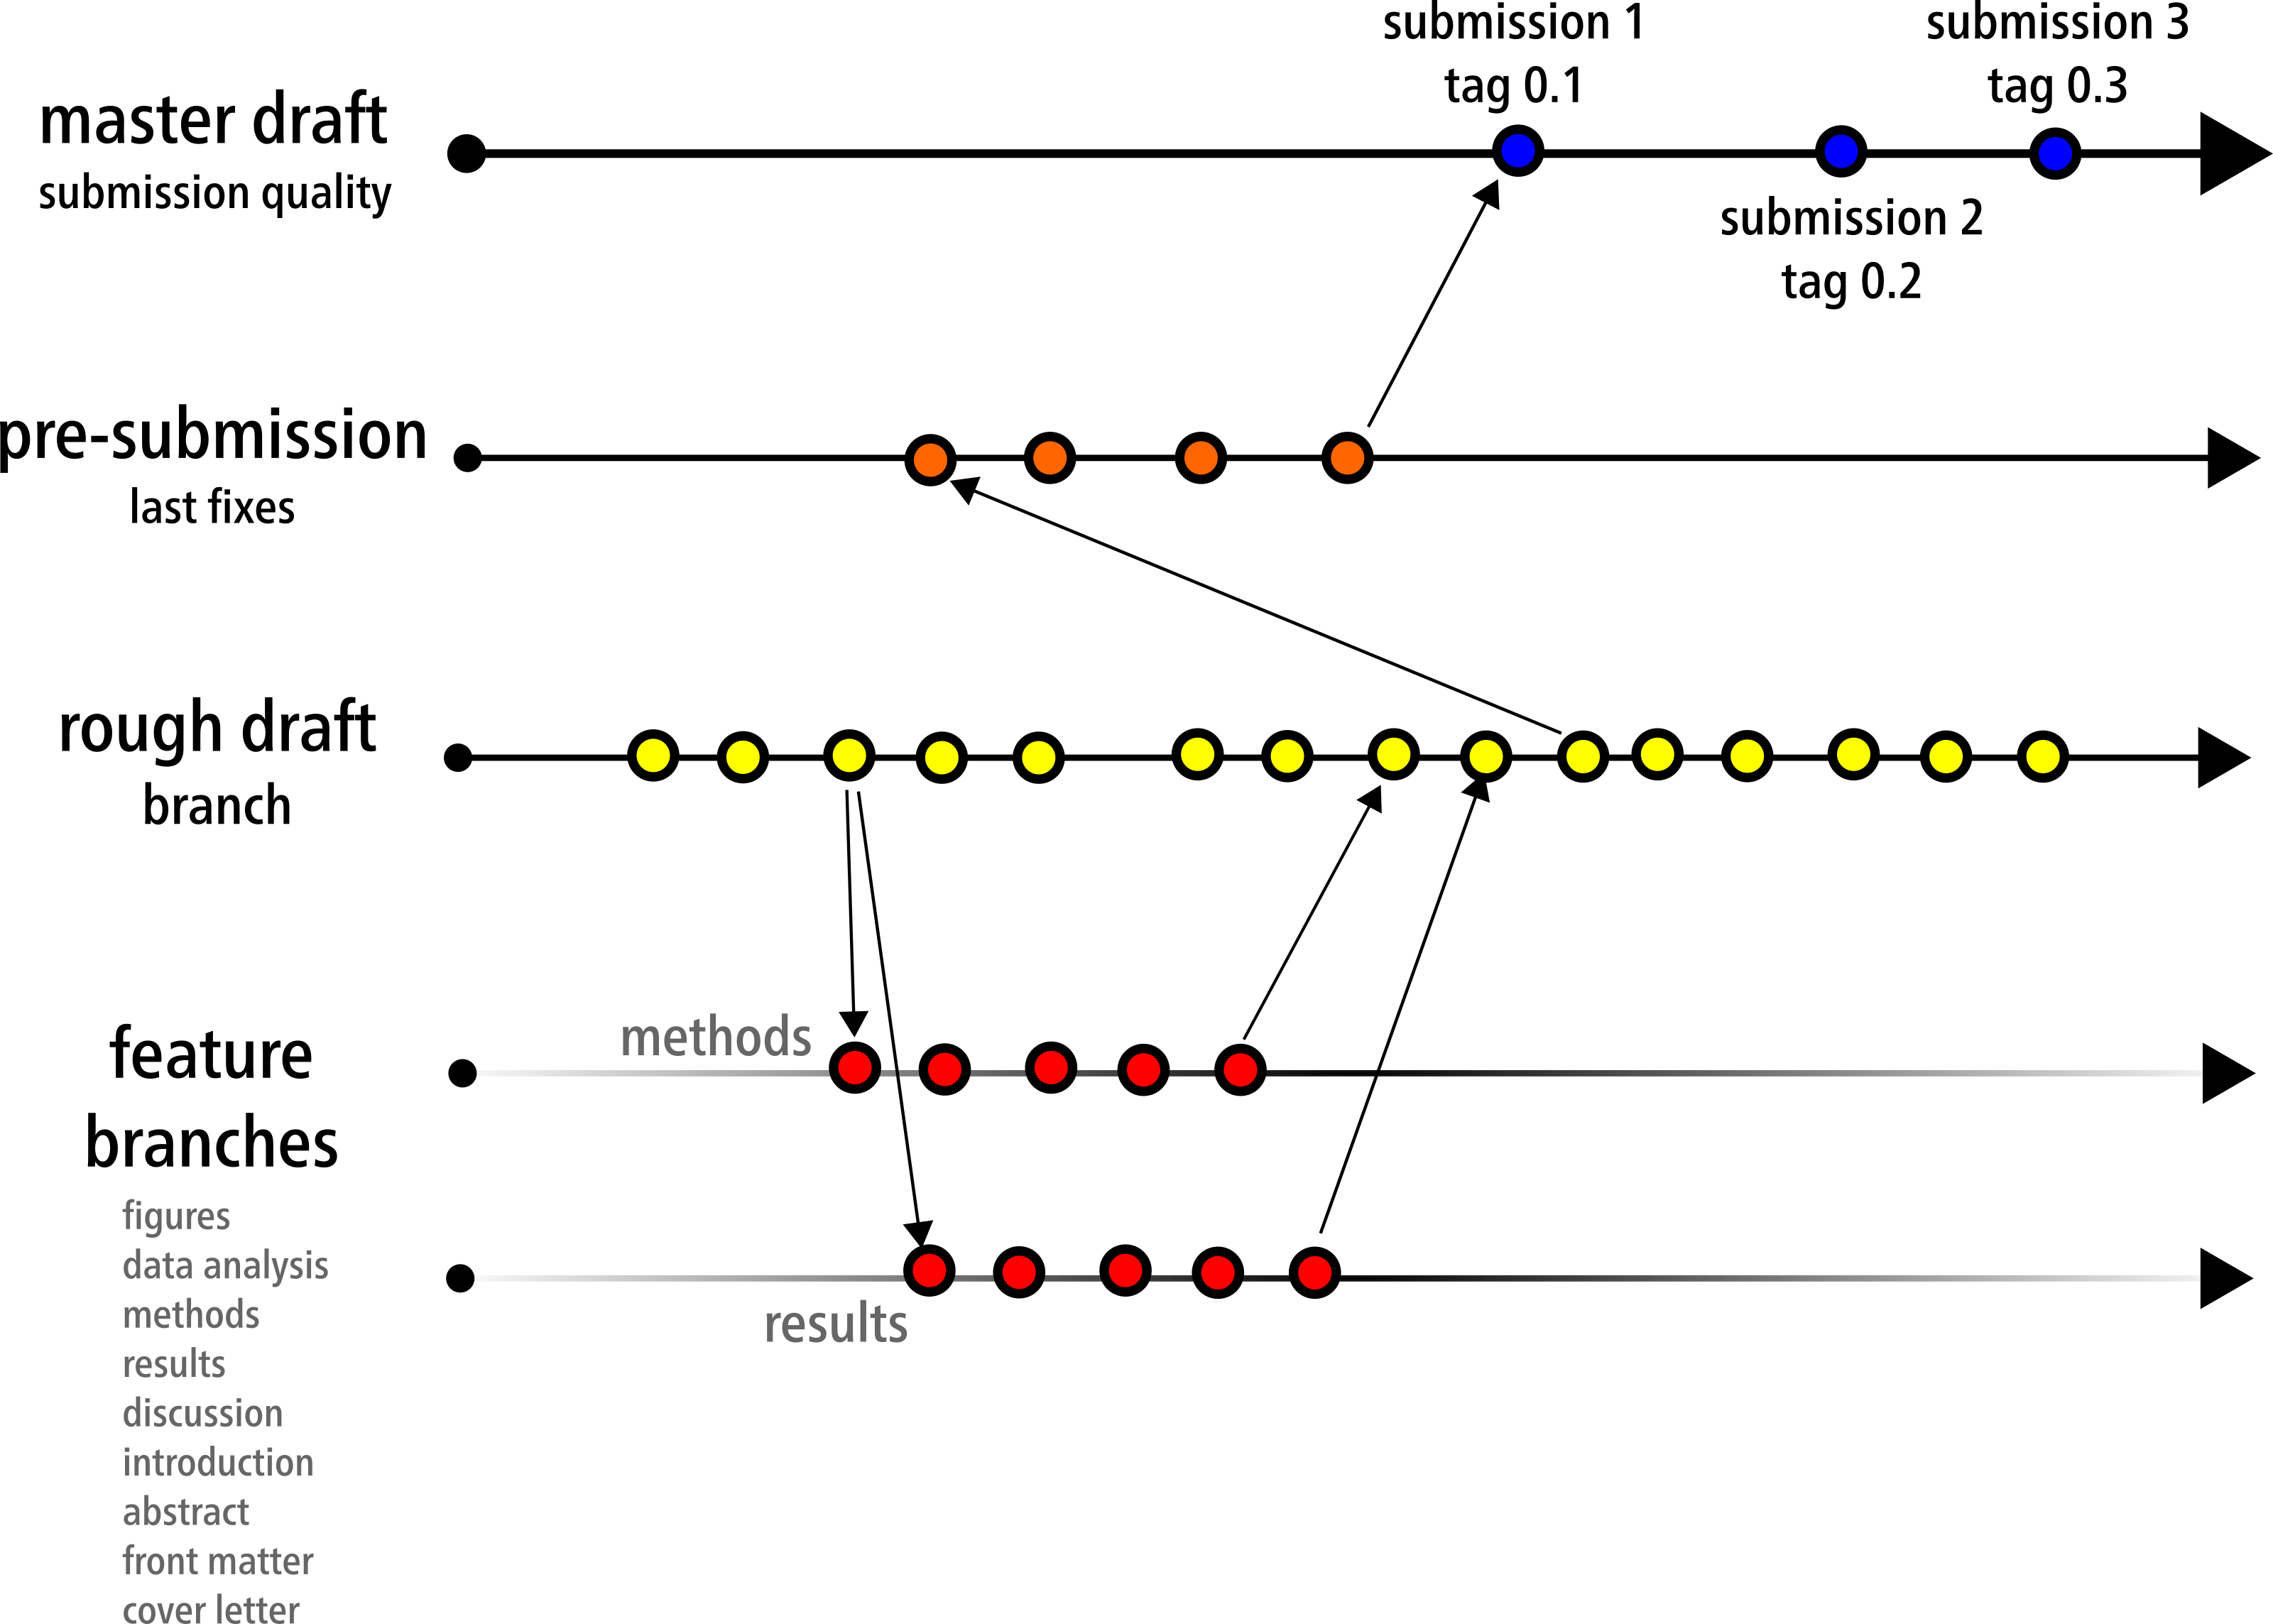
\includegraphics{images/GitFlow-Science.png}
\caption{GitFlow for development of a Research Manuscript}
\end{figure}

\section{Main branches}\label{main-branches}

The central repo holds two branches with an infinite lifetime:

\begin{itemize}
\tightlist
\item
  \texttt{master} (publication ready state)
\item
  \texttt{rough-draft} (latest delivered development state)
\end{itemize}

When \texttt{rough-draft} branch is reached stable state suitable for
submission to a journal, all of the changes are merged into
\texttt{master} branch and tagged with a manuscript release number.

\section{Supporting branches}\label{supporting-branches}

Supporting branches have limited life time and will be removed
eventually.

Two different types of branches we may use:

\begin{itemize}
\tightlist
\item
  Feature branches
\item
  Pre-submission branches
\end{itemize}

\subsection{Feature branches}\label{feature-branches}

Feature branches are used to develop a specific part of the manuscript.
These are the branches where the most work is done by the members of the
team. These branches are created locally on the machines where these
features are being develop and they are merged through Pull requests
only into rough-draft branch. These branches are short lived and will
follow the following convention:

May branch off from:

\begin{itemize}
\tightlist
\item
  \texttt{rough-draft}
\end{itemize}

Must merge back into:

\begin{itemize}
\tightlist
\item
  \texttt{rough-draft}
\end{itemize}

Branch naming convention:

\begin{itemize}
\tightlist
\item
  anything except master, rough draft, pre-submission
\end{itemize}

\subsubsection{Creating a feature
branch}\label{creating-a-feature-branch}

When starting work on a new feature, branch off from the
\texttt{rough-draft} branch.

\begin{quote}
\$ git checkout -b myfeature rough-draft
\end{quote}

\begin{quote}
Switched to a new branch ``myfeature''`
\end{quote}

\subsubsection{Incorporating a finished feature on
develop}\label{incorporating-a-finished-feature-on-develop}

Finished features may be merged into the develop branch to definitely
add them to the upcoming release:

\begin{quote}
\$ git checkout develop
\end{quote}

\begin{quote}
Switched to branch `develop'
\end{quote}

\begin{quote}
\$ git merge --no-ff myfeature
\end{quote}

\begin{quote}
Updating ea1b82a..05e9557
\end{quote}

\begin{quote}
(Summary of changes)
\end{quote}

\begin{quote}
\$ git branch -d myfeature
\end{quote}

\begin{quote}
Deleted branch myfeature (was 05e9557).
\end{quote}

\begin{quote}
\$ git push origin develop
\end{quote}

The \texttt{-\/-no-ff} flag causes the merge to always create a new
commit object, even if the merge could be performed with a fast-forward.
This avoids losing information about the historical existence of a
feature branch and groups together all commits that together added the
feature.

In the latter case, it is impossible to see from the Git history which
of the commit objects together have implemented a feature---you would
have to manually read all the log messages. Reverting a whole feature
(i.e.~a group of commits), is a true headache in the latter situation,
whereas it is easily done if the --no-ff flag was used.

Yes, it will create a few more (empty) commit objects, but the gain is
much bigger than the cost.

\subsection{Pre-submission branch}\label{pre-submission-branch}

May branch off from:

\texttt{rough-draft}

Must merge back into:

\texttt{master}

Branch naming convention:

\texttt{pre-submission*}

This branch is to bring a complete rough draft to a specific publication
standard. Various journals will have variuos requirements. This branch
will branch of a complete rough-draft and will merge only into master. A
submission will be residing in the master branch.

\subsubsection{Creating pre-submission
branch}\label{creating-pre-submission-branch}

\begin{quote}
\$ git checkout -b \texttt{presubmission} rough-draft
\end{quote}

\begin{quote}
Switched to a new branch ``presubmission''
\end{quote}

\begin{quote}
\$ ./bump-version.sh 0.1
\end{quote}

\begin{quote}
Files modified successfully, manuscript version bumped to 0.1.
\end{quote}

\begin{quote}
\$ git commit -a -m ``Bumped manuscript version number to 0.1''
\end{quote}

\begin{quote}
{[}presubmission 41e61bb{]} Bumped version number to 0.1
\end{quote}

\begin{quote}
1 files changed, 1 insertions(+), 1 deletions(-)
\end{quote}

Don't forget to bump the version number after branching off!

Then, bring the manuscript to a submission ready state in one or more
separate commits.

\begin{quote}
\$ git commit -m ``Manuscript is brought to submission ready state for
sumbmission in \ldots{}''
\end{quote}

\begin{quote}
{[}presubmission abbe5d6{]} Manuscript is brought to submission ready
state for sumbmission in \ldots{}
\end{quote}

\begin{quote}
5 files changed, 32 insertions(+), 17 deletions(-)
\end{quote}

\paragraph{Finishing presubmission
branch}\label{finishing-presubmission-branch}

When finished, the \texttt{presubmission} branch needs to be merged into
\texttt{master}.

First, update master and tag the release.

\begin{quote}
\$ git checkout master
\end{quote}

\begin{quote}
\begin{verbatim}
  Switched to branch 'master'
\end{verbatim}
\end{quote}

\begin{quote}
\$ git merge --no-ff presubmission
\end{quote}

\begin{quote}
\begin{verbatim}
  Merge made by recursive.
\end{verbatim}
\end{quote}

\begin{quote}
\begin{verbatim}
  (Summary of changes)
\end{verbatim}
\end{quote}

\begin{quote}
\$ git tag -a 0.1
\end{quote}

Finally, remove the temporary \texttt{presubmission} branch:

\begin{quote}
\$ git branch -d presubmission
\end{quote}

\begin{quote}
\begin{verbatim}
  Deleted branch presubmission (was abbe5d6).
\end{verbatim}
\end{quote}

\chapter{Data Visualization}\label{data-visualization}

\chapter{Data Analysis}\label{data-analysis}

\chapter{Project Organization}\label{project-organization}

\chapter{Manuscript Template}\label{manuscript-template}

\chapter{Supplemental Materials}\label{supplemental-materials}

\chapter{Manuscript Submission}\label{manuscript-submission}

\bibliography{packages,book}


\end{document}
